% -------------------------------------------------------------------------------- %

\begin{exercise}[Point estimator statistics: Comparison]

Let $X_1, \dots, X_n$ be i.i.d. uniform $(0, \theta)$, with unknown parameter $\theta > 0$.

\begin{enumerate}[label = (\alph*)]

    \item Show that the method of moments estimator of $\theta$ is $2 \bar X$ and the MLE of $\theta$ is $X_{(n)} = \max_{1 \leq i \leq n} X_i$.

    \item Compare the mean square errors of the two estimators.
    Which of the estimators should be preferred if any?
    Explain your reasoning.

\end{enumerate}

\end{exercise}

% -------------------------------------------------------------------------------- %

\begin{solution}

\phantom{}

\begin{enumerate}[label = (\alph*)]

    \item

    \begin{enumerate}[label = (\roman*)]

        \item 

        \begin{align*}
            \frac{\hat \theta}{2} = \E_{\hat \theta} X_1 \stackrel{!}{=} \frac{1}{n} \sum_{i=1}^n X_i = \bar X
            \iff
            \hat \theta = 2 \bar X
        \end{align*}

        \item This was already done in \cite[lecture 6, slides 68-69]{EStat}.

        \includepdf[
            pages = {69, 69},
            nup = 1x2
        ]
        {../../../EStat_VO/Lecture Slides/Lecture 6.pdf}

    \end{enumerate}

    \item

    \begin{enumerate}[label = \arabic*.]

        \item MSE:
        
        \begin{align*}
            \E(2 \bar X)
            & =
            \E \pbraces{\frac{2}{n} \sum_{i=1}^n X_i} \\
            & =
            \frac{2}{n}
            \sum_{i=1}^n \E X_i \\
            & =
            \frac{2}{n}
            \sum_{i=1}^n
                \frac{\theta}{2} \\
            & =
            \frac{2}{n}
            \frac{\theta}{2}
            n \\
            & =
            \theta
        \end{align*}
        
        \begin{align*}
            \Var(2 \hat X)
            & =
            \Var \pbraces{\frac{2}{n} \sum_{i=1}^n X_i} \\
            & =
            \frac{4}{n^2}
            \sum_{i=1}^n
                \Var X_i \\
            & =
            \frac{4}{n^2}
            \sum_{i=1}^n
                \frac{\theta^2}{12} \\
            & =
            \frac{4}{n^2}
            \frac{\theta^2}{12}
            n \\
            & =
            \frac{\theta^2}{3 n}
        \end{align*}

        \begin{align*}
            \MSE(2 \bar X)
            =
            \E(2 \bar X - \theta)^2
            =
            \Var(2 \bar X) + b^2(2 \bar X)
            =
            \frac{\theta^2}{3 n}
        \end{align*}

        \item MSE:
        
        From \cite[lecture 5, slide 88]{EStat}, we take

        \begin{align*}
            f_{X_{(n)}}(x)
            & =
            \frac{n!}{(n-1!) (n-n)!} F_{X_1}(x)^{n-1} (1 - F_{X_1}(x))^{n-n} f_{X_1}(x) \\
            & =
            n \pbraces{\frac{x}{\theta}}^{n-1} \frac{1}{\theta} \mathbf 1_{(0, \theta)}(x) \\
            & =
            \frac{n x^{n-1}}{\theta^n} \mathbf 1_{(0, \theta)}(x).
        \end{align*}

        \begin{align*}
            \E X_{(n)}
            & =
            \Int[-\infty][\infty]
            {
                x f_{X_{(n)}}(x)
            }{x} \\
            & =            
            \Int[-\infty][\infty]
            {
                x \frac{n x^{n-1}}{\theta^n} \mathbf 1_{0, \theta}(x)
            }{x} \\
            & =
            \frac{n}{\theta^n}
            \Int[0][\theta]
            {
                x^n
            }{x} \\
            & =
            \frac{n}{\theta^n}
            \frac{\theta^{n+1}}{n+1} \\
            & =
            \frac{n}{n+1} \theta
        \end{align*}

        \begin{align*}
            b(X_{(n)})
            & =
            \E X_{(n)} - \theta \\
            & =
            \frac{n}{n+1} \theta - \theta \\
            & =
            \pbraces
            {
                \frac{n}{n+1} - 1
            }
            \theta \\
            & =
            \frac{n - (n+1)}{n+1} \theta \\
            & =
            -\frac{\theta}{n+1}
        \end{align*}

        \begin{align*}
            \E X_{(n)}^2
            & =
            \Int[-\infty][\infty]
            {
                x^2 f_{X_{(n)}}
            }{x} \\
            & =
            \Int[-\infty][\infty]
            {
                x^2 \frac{n x^{n-1}}{\theta^n} \mathbf 1_{0, \theta}(x)
            }{x} \\
            & =
            \frac{n}{\theta^n}
            \Int[0][\theta]
            {
                x^{n+1}
            }{x} \\
            & =
            \frac{n}{\theta^n}
            \frac{\theta^{n+2}}{n+2} \\
            & =
            \frac{n}{n+2} \theta^2
        \end{align*}

        \begin{align*}
            \Var X_{(n)}
            & =
            \E X_{(n)}^2 - \E^2 X_{(n)} \\
            & =
            \frac{n}{n+2} \theta^2 - \pbraces{\frac{n}{n+1} \theta}^2
        \end{align*}

        \begin{align*}
            \MSE(X_{(n)})
            & =
            \E (X_{(n)} - \theta)^2 \\
            & =
            \Var X_{(n)} + b^2(X_{(n)}) \\
            & =
            \frac{n}{n+2} \theta^2 - \pbraces{\frac{n}{n+1} \theta}^2
            +
            \pbraces
            {
                -\frac{\theta}{n+1}
            }^2 \\
            & =
            \frac{n}{n + 2} \theta^2
            -
            \frac{n^2}{(n + 1)^2} \theta^2
            +
            \frac{1}{(n + 1)^2} \theta^2 \\
            & =
            \pbraces
            {
                \frac{n}{n + 2} - \frac{n^2 - 1}{(n + 1)^2}
            }
            \theta^2 \\
            & =
            \pbraces
            {
                \frac{n}{n + 2}
                -
                \frac{(n + 1) (n - 1)}{(n + 1)^2}
            }
            \theta^2 \\
            & =
            \pbraces
            {
                \frac{n}{n + 2}
                -
                \frac{n - 1}{n + 1}
            }
            \theta^2 \\
            & =
            \frac{n (n + 1) - (n - 1) (n + 2)}{(n + 1) (n + 2)} \theta^2 \\
            & =
            \frac{n^2 + n - n^2 - 2 n + n + 2}{(n + 1) (n + 2)} \theta^2 \\
            & =
            \frac{2}{(n + 1) (n + 2)} \theta^2
        \end{align*}

    \end{enumerate}

    Overall, we have

    \begin{align*}
        \MSE(2 \bar X) = \theta^2 \Landau(n^{-1}),
        \quad
        \MSE(X_{(n)}) = \theta^2 \Landau(n^{-2}).
    \end{align*}

    Because the $\MSE$ of $X_{(n)}$ converges to $0$ faster, $X_{(n)}$ ist probably better than $2 \bar X$.

\end{enumerate}

\end{solution}

% -------------------------------------------------------------------------------- %
